%
% Example Workshop Handout with title page and a section demonstrating
% the different environments defined in the top matter
%
\documentclass[a4paper,12pt,twoside]{memoir}
\usepackage{btp}    % Use the trainermanual package option (i.e. \usepackage[trainermanual]{btp}) to generate the Trainer's version of the manual
\usepackage{url}
\usepackage{underscore}
\usepackage{color}

% Enable line breaks after every alphabetic character in the url package
\expandafter\def\expandafter\UrlBreaks\expandafter{\UrlBreaks \do\a\do\b\do\c\do\d\do\e\do\f\do\g\do\h\do\i\do\j\do\k\do\l\do\m\do\n\do\o\do\p\do\q\do\r\do\s\do\t\do\u\do\v\do\w\do\x\do\y\do\z\do\A\do\B\do\C\do\D\do\E\do\F\do\G\do\H\do\I\do\J\do\K\do\L\do\M\do\N\do\O\do\P\do\Q\do\R\do\S\do\T\do\U\do\V\do\W\do\X\do\Y\do\Z}

\usepackage{graphicx}
\DeclareGraphicsExtensions{.pdf,.png,.jpg}
\graphicspath{ {./images/} }

\usepackage[T1]{fontenc}
\newcommand{\spCite}[1]{\textsuperscript{\cite{#1}}}

% Set some Workshop specific info
\setWorkshopTitle{Introduction To NGS Data \& Analytic Tools}
\setWorkshopVenue{Adelaide, South Australa}
\setWorkshopDate{October 2014}
\setWorkshopAuthor{Steve Pederson\\
Bioinformatics Centre\\
University Of Adelaide}


\begin{document}

%
% Workshop Title Page
%
\workshoptitlepage

\chapter{Introduction}

Thank you for your attendance \& welcome to the Introduction to NGS Data \& NGS Analytic Tools Workshop.
This is a free offering by the University of Adelaide, Bioinformatics Hub which is a centrally funded initiative from the Department of Vice-Chancellor (Research), with the aim of assisting \& enabling researchers in their work.
Training workshops \& seminars such as this one  are an important part of this initiative. \\

The Bioinformatics Hub itself has a web-page at \url{http://www.adelaide.edu.au/bioinformatics-hub/}, and to be kept up to date on upcoming events and workshops, please join the internal Bioinformatics mailing list on \url{http://list.adelaide.edu.au/mailman/listinfo/bioinfo}.\\

Today's workshop has been prepared with generous technical support \& advice provided by Dr Nathan Watson-Haigh (\textit{ACPFG}), Dr Dan Kortschak (\textit{Adelaide University, Adelson Research Group}), Dr Zhipeng Qu (\textit{Adelaide University, Adelson Research Group}), Dr Mark Corbett (\textit{Robinson Institute}) \& Dr John Toubia (\textit{Adelaide Centre for Cancer Genomics}). 
The tutors today are Steve Pederson (\textit{Adelaide University, Bioinformatics Hub}), Dr John Toubia, \& Dr Terry Bertozzi (\textit{SA Museum \& Adelaide University, Adelson Research Group}). 
We hope it will be useful in enabling you to continue and to advance your research.\\

\section{Course Summary}
In today's workshop we will be introducing you to a small number of the basic tools required for NGS data handling, as well as giving you a basic familiarity with what the data actually looks like.
Whilst we will not be able to cover all of the rich \& diverse set of tools available, we hope to cover many of the key concepts \& questions to ask of your data, as well as give you an understanding of what information is actually in the data.\\

The majority of data handling and analysis required in the field of bioinformatics uses the \textit{command line}, alternatively known as the terminal or the \textit{bash shell}, so some useful tips for the command line will be included amongst the material.
Whilst most of the session will involve looking at individual files, in reality most of our analysis will be performed using some type of script to automate, \& easily reproduce an analysis. \\

Today's session is also intended to explore several tools in actual detail, rather than rush across the whole field.
There is large amount of information that we won't have time to discuss, but hopefully some important tools and thought processes will be covered \& enable you make better progress with your own datasets.\\

\section{Post Workshop}
The VMs which we work on today will remain active for week or so after the workshop, so feel free to continue exploring any sections that you weren't able to make it through.
We'd also encourage you to sign up for some of the high-traffic websites like \textit{BioStars} or \textit{SEQanswers} as these are a rich resource for your own problem solving.

\section{Icons \& Symbols}
The following set of symbols will be used throughout this document to assist you finding your way: \\

\begin{information}
Important information.\\
\end{information}

\begin{note}
Things to note.\\
\end{note}

\begin{warning}
A warning which needs to be read very carefully.\\
\end{warning}

\begin{steps}
Instructions for you to perform. \\
\end{steps}

\begin{questions}
Questions for you to answer. \\
\begin{answer}
There is no answer
\end{answer}
\end{questions}

\begin{bonus}
An optional bonus section for those progressing rapidly. \\
\end{bonus}

\begin{advanced}
An optional advanced section for those progressing very rapidly or to be used for future reference. \\
\end{advanced}

\section{Using NoMachine} \label{sec:NoMachine}
\begin{information}
We will all be working on our own computers today, and will be accessing Virtual Machines running the Ubuntu operating system on the Nectar Research Cloud (\url{http://nectar.org.au/}).
The software client NoMachine which you will have already installed, enables us to access these machines in a familiar Desktop style, even though the majority of our time will be spent within the terminal. \\

NoMachine session files will be provided to everyone which have been pre-configured to enable easy access to these machines.
\textbf{If you attended last weeks session, please use the same VM connection}.
These machines are effectively dual-core machine with 8GB of RAM \& 70GB of hard drive space.
Whilst relatively small, this will be more than enough to become familiar with the important concepts for the day.
To begin today's session, simply click (or double-click) on the NoMachine session file that you have been given.
The desktop from the Virtual Machine (VM) that you have connected to will appear on the NoMachine client. \\
\end{information}

\begin{figure}[h!]
  \centering
    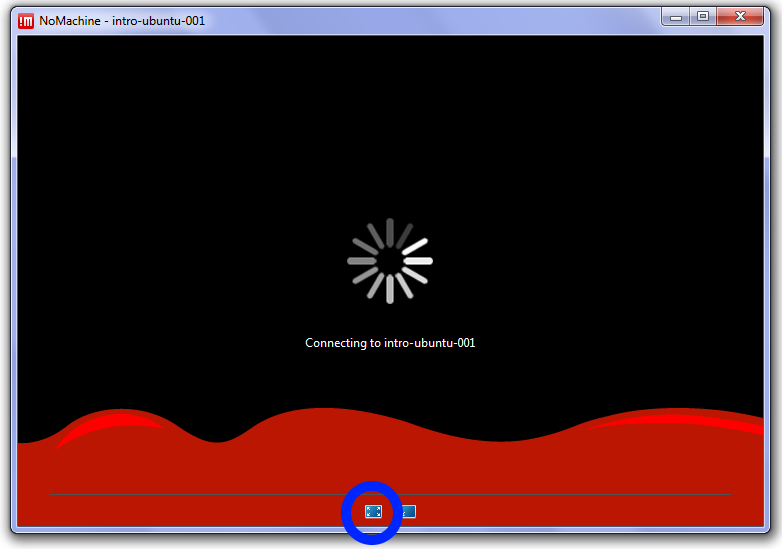
\includegraphics[width=0.8\textwidth]{NoMachine}
\end{figure}

\begin{information}
While this is connecting, select the button circled in blue above.
This will resize NoMachine to be full screen to feel more like you are physically located at the VM.
If any security warnings appear, ignore them \& continue connecting. 
It can be a little temperamental, but if connection using NoMachine fails after a few attempts, let us know \& we'll be able to get you going.\\
\end{information}

\begin{information}
Once connected to the VM, \textit{hovering your mouse over the top right corner of the screen will cause the corner of the screen to ``fold over".}
If you click in the corner of this, the main control settings for NoMachine will appear.
Here you can change in \& out of the full screen setting, and you can also select the connection page to disconnect from the VM at the end of the session.
\end{information}

\section{The Ubuntu Desktop}
\begin{note}
Now that you are connected, you will notice we are in a standard graphical environment.
The default Desktop in Ubuntu is Unity, but what we are seeing is known as the Gnome Desktop, as is the default for Nectar VMs.
As many of us are used to seeing, there are click-able icons on the desktop, and drop-down menus. \\

The main interfaces we will be using today are the \texttt{terminal}, a text editor named \texttt{gedit} and the web browser \texttt{firefox}
They will appear as icons on the desktop, but can also be accessed from the drop-down menus.
A \texttt{Firefox} icon is also located on the desktop \& this can be used for searching for answers as well as viewing the output of \texttt{fastqc}.
%When viewing clips  you will be unable to obtain sound from the VM, so switch back to your normal laptop for these.
\end{note}

\subsection{Basic Shell Comands}
\begin{note}
Today we will assume a basic familiarity with the bash terminal in Linux.
Some key commands which we will be using are explained in the following table.
\end{note}
\begin{center}
  \begin{tabular}[h]{|p{3cm} | p{11.5cm} |}
    \hline
    \textbf{Command} & \textbf{Meaning} \\
    \hline
    \texttt{cd} & Change directory \\
    \texttt{ls} & List files in a directory \\
    \texttt{man} & Call the manual for a given command \\
    \texttt{head} & View the first 10 lines of a file \\
    \hline
  \end{tabular}
\end{center}

\begin{steps}
Open a terminal in the VM by either clicking on the icon, or using the drop-down menu.
It will automatically open in your home directory (\texttt{/home/trainee}), which is indicated by the tilde before the dollar sign.
The tilde (\~{}) is a symbolic representation of the address \texttt{/home/trainee}, where the first slash is the root of the computer’s file system.
To return to this directory from any other in the file system, you can simply enter the command
\begin{lstlisting}
cd 
\end{lstlisting}
\end{steps}


Normally we specify the directory to change into after the command \texttt{cd}, but when no directory is given, this command will automatically change to your home directory.\\

\begin{warning}
Please note, the Linux operating system is case-sensitive.
When entering the any commands, please make sure that you pay attention to this detail.
Spaces are an important feature as well, so be careful not to add or omit them where they appear in any sample code.
\end{warning}

\section{Today's Data}
\begin{steps}
The raw data for today's workshop is in the directory \texttt{/home/trainee/rawData}.
Change into this directory \& have a look at the files in the directory by entering the following.
\begin{lstlisting}
cd ~/NGSData
ls -lhR
\end{lstlisting}
\end{steps}

After the \texttt{ls} command we specified the options \texttt{l}, \texttt{h} \& \texttt{R} by including them after the dash.
The first two of these set the output of the command to be in \textit{\underline{l}ong listing} format, and change the filesize to be output in ``\textit{\underline{h}uman-readable} format", which really means that sizes are stated in Mb or Gb, instead of bytes.
(You can try it without the \texttt{h} if you're curious.)
The \texttt{R} option allowed the command to operate \textit{\underline{r}ecursively} through the directories within \texttt{\~{}/NGSData}.
The list of options available for this command can be found using the command
\begin{lstlisting}
man ls
\end{lstlisting}
This command will open the help page in a program known as the \textit{less} pager, which makes your terminal into a text reader.
Scroll down by using the \textless \texttt{space bar}\textgreater \ until you find these two options to see what they mean.
You can navigate back a page by hitting the \textless \texttt{b}\textgreater \ key.
Exit the less pager when you are finished by entering \textless \texttt{q}\textgreater .
\clearpage
\chapter{NGS Data \& Quality Assessment}

\section{Initial Goals}

\begin{enumerate}
\item Understand the \textit{Sequencing by Synthesis} Process \& Data Generation \\
\item Understand what errors and artefacts lie within the data \\
\item Learn how to assess the quality of data \& make informed decisions \\
\end{enumerate}

\section{NGS Data Generation}
\begin{steps}
Before we can begin to analyse any data, it is helpful to understand how it was generated.
Whilst there are numerous platforms for generation of NGS data, today we will look at the Illumina \textit{Sequencing by Synthesis} method, which is one of the most common methods in use today.
Many of you will be familiar with the process involved, but it may be worth looking at the following 5-minute video from Illumina: \url{http://youtu.be/womKfikWlxM} 
As setting up the sound with the VMs can be tricky, it will be easier to view this from your own regular browser.
Briefly minimise the VM (see Section 1.4), open your regular browser \& please use your headphones if you brought them. \\
\end{steps}

\begin{note}
This video refers to the process \textit{tagmentation}.
This is a relatively recent method for fragmenting \& attaching adaptors to DNA, with an alternative, more traditional method being sonication, poly-adenylation \& attachment of appropriate adaptors in separate steps.
\end{note}

\begin{information}
The important concept to note during sample preparation is that the DNA insert has multiple sequences ligated to either end.
These include 1) the \textit{sequencing primers}, 2) index or \textit{barcode} sequences, and 3) the flow-cell binding oligos.
\end{information}

\begin{questions}
Assuming each 'spot' on the flowcell is generated from a unique DNA sequence, there are two important sequencing errors that will occur during this process.
What do you think they might be? \\
\begin{answer}
1) Ligation of the wrong base during sequencing \\
2) Insertions \& deletions \\
It's the same basic errors as normal DNA replication, but without the \textit{in vivo} DNA repair mechanisms.
\end{answer}

Will these errors have a more significant effect if they occur during the sequence detection stage, or during generation of the DNA clones within each cluster? \\
\begin{answer}
The earlier in the process any sequencing errors occur, the higher the degree to which they will be propagated.
If an error occurs during the very first round of amplification, before even bridge amplification, it will be propagated through an entire cluster. \\
\end{answer}
\end{questions}

\section{FASTQ File Format}
\begin{note}
As the sequences are extended during the sequencing reaction, an image is recorded which is effectively a movie or series of frames at which the addition of bases is recorded \& detected.
We mostly don't deal with these image files, but will handle data generated from these in \textit{fastq} format, which can commonly have the file suffix \textit{.fq} or \textit{.fastq}.
As these files are often very large, they will often be zipped using \texttt{gzip} or \texttt{bzip}.
Whilst we would instinctively want to unzip these files using the command \texttt{gunzip}, most NGS tools are able to work with zipped fastq files.
This can save considerable hard drive space, which is an important consideration when handling NGS datasets as the quantity of data can easily push your storage capacity to it's limit. \\
\end{note}

\begin{steps}
We should still have a terminal open from the previous section \&, if necessary, use the \texttt{cd} command to make sure you are in the \texttt{\~{}/rawData/RNASeq} directory.
The command \texttt{zcat} unzips a file \& prints the output to the terminal, or standard output (\textit{stdout}).
If we did this to these files, we would see a stream of data whizzing past in the terminal, but instead we can just pipe the output of \texttt{zcat} to the command head to view the first 10 lines of a file. \\
\begin{lstlisting}
zcat reads1.fq.gz | head
\end{lstlisting}
\end{steps}

\begin{information}
In the above command, we have used a trick commonly used in Linux systems where we have taken the output of one command (\texttt{zcat reads1.fq.gz}) and sent it to another command (\texttt{head}) by using the \textit{pipe symbol} (|).
This is literally like sticking a pipe on the end of a process \& redirecting the output to the input another process.
If you think of things as being like a data factory you can almost visualise it.
There are no limits to the number of commands that you can string together using this trick. \\
\end{information}

\begin{warning}
\large{Don't Panic!!!} \\
\normalsize
If at some stage today you find that the terminal has become unresponsive, or you are seeing an unexpected stream of data fly past, you can abort whichever process is currently running in the terminal by entering \texttt{Ctrl-c}.
This is an instruction to the computer to `kill the current process.' \& you may be surprised at how often this comes in handy.
Even experienced programmers rely on this trick from time to time.
\end{warning}

\begin{note}
In the output from the above terminal command, we have obtained the first 10 lines of the gzipped fastq file.
This gives a clear view of the fastq file format, where each individual read spans four lines.
These lines are:
\begin{enumerate}
\item The read identifier
\item The sequence read
\item An alternate line for the identifier (commonly left blank as just a \texttt{+} symbol
\item The quality scores for each position along the read
\end{enumerate}
\end{note}

\subsubsection*{The read identifier}
This line begins with an \texttt{@} symbol and although there is some variability, it traditionally has several components.
Today's data have been sourced from an EBI data repository with the identifier \texttt{SRR031714}.
For the first sequence in this file, we have the full identifier \texttt{@SRR031714.1 HWI-EAS299_130MNEAAXX:2:1:785:591/1} which has the following components \\

\begin{tabular}{|p{5cm} | p{9cm} |}
  \hline
  \texttt{SRR031714.1} & The aforementioned EBI identifier \& the sequence ID within the file. As this is the first read, we have the number 1. NB: This identifier is \textbf{not} present when data is obtained directly from the machine or service provider.\\
  \hline
  \texttt{WHI-EAS299_130MNEAAXX} & The unique machine ID \\
  \hline
  \texttt{2} & The flowcell lane \\
  \hline
  \texttt{1} & The tile within the flowcell lane \\
  \hline
  \texttt{785} & The $x$-coordinate of the cluster within the tile \\
  \hline
  \texttt{591} & The $y$-coordinate of the cluster within the tile \\
  \hline
  \texttt{/1} & Indicates that this is the first read in a set of paired end reads \\
  \hline
\end{tabular}

As seen in the subsequent sections, these pieces of information can be helpful in identifying if any spatial effects have affected the quality of the reads.\\

\begin{steps}
While we are inspecting our data, have a look at the beginning of the second file.
\begin{lstlisting}
zcat reads2.fq.gz | head
\end{lstlisting}
Here you will notice that the information in the identifier is identical to the first file we inspected, with the exception that there is a \texttt{/2} at the end.
This indicates that these reads are the second set in what are known as \textit{paired-end} reads, as were introduced in the above video.
The two files will have this identical structure where the order of the sequences in one is identical to the order of the sequences in the other.
This way when they are read as a pair, they can be stepped through read-by-read \& the integrity of the data will be intact.
\end{steps}


\subsubsection{The Illumina Chastity Filter}
\begin{information}
It is also worth noting that the reads we've just glanced at come from a version of the Illumina \textit{casava} pipeline which is \textless 1.8, and which is a relatively common format.
For more recently generated reads which have used \textgreater 1.8 of the casava pipeline, there is an additional field in the identifier which indicates whether a read would have \textit{failed} an initial QC check. 
An example of this format would be:
\begin{lstlisting}
@D5B4KKQ1:554:C4YHPACXX:4:1101:1084:2100 1:Y:0:
\end{lstlisting}
Note the ``Y'' in the final fields, which indicates this sequence would have failed QC.
These low-quality reads were automatically removed in early versions of the pipeline and were omitted from the fastq file.
However, they are now included with this additional field indicated in the read identifier.
Inspection of the read identifiers will enable you to find out which version of the casava pipeline has been used, and whther you need to perform any additional filtering steps to remove low quality reads. 
The tool \texttt{fastq_illumina_filter} is designed to remove these reads for you \& the tool, along with usage instructions can be found at \url{http://cancan.cshl.edu/labmembers/gordon/fastq_illumina_filter/}\\
\end{information}

\begin{steps}
An alternate set of reads which we'll also explore today is in included in the directory \texttt{\~{}/rawData/iCLIP}.
These are immunopreciptated mRNAs and were supplied by some collaborators who'd either forgotten the removal of low-quality reads or had deliberately neglected step to increase read numbers.
Note that these files are not compressed and are essentially plain text files, so we can inspect them using the command \texttt{head}.\\
\end{steps}

\begin{lstlisting}
cd ~/rawData/iCLIP
head -n12 iCLIP_Sample1.fastq
\end{lstlisting}

Note that the header lines follow the format described on the previous page with this additional field at the end of the line.
\begin{questions}
Of the first three reads which have been printed to the terminal above, which one(s) will have failed the chastity filter, and which ones will have passed the filter?\\
\begin{answer}
The first read would have failed (i.e. it is low quality), whilst the other two will have passed.
\end{answer}
\end{questions}

\subsubsection{Quality Scores}
\begin{information}
The only other line in the fastq format that really needs some introduction is the quality score information.
These are presented as single \textit{ascii} text characters for simple visual alignment with the sequence and each character corresponds to a numeric score.
In the ascii text system, each character has a representation in binary, which can also be translated to decimal numbers.\\

The first printable character in the ascii system is `!' which corresponds to the value 33. 
(A space is also considered printable and has the value 32, but we can ignore that)
In short, the values 33-47 are symbols like !, \", \#, \$ etc, whereas the values 48-57 are the characters 0-9.
Next are some more symbols (including @ for the value 64), with the upper case characters representing the values 65-90 \& the lower case letters representing the values 97-122.
For a full list of ascii characters see \url{http://en.wikipedia.org/wiki/ASCII#ASCII_printable_code_chart}.
\end{information}

\subsubsection{The PHRED +33/64 Scoring System}
\begin{information}
Now that we understand how to turn the quality scores from an ascii character into a numeric value, we need to know what these numbers represent.
The two main systems in common usage are PHRED +33 and PHRED +64 and for each of these coding systems we either subtract 33 or 64 from the numeric value associated with each ascii character to give us a PHRED score (or Q-value)
For example, in PHRED +33, the @ symbol corresponds to Q = 64 - 33 = 31, whereas in PHRED +64 it corresponds to Q = 64 - 64 = 0. \\
\end{information}

The following table demonstrates the comparative coding scale for the different formats: \\

\scriptsize
\texttt{SSSSSSSSSSSSSSSSSSSSSSSSSSSSSSSSSSSSSSSSS..................................................... \\
..........................XXXXXXXXXXXXXXXXXXXXXXXXXXXXXXXXXXXXXXXXXXXXXX...................... \\
...............................IIIIIIIIIIIIIIIIIIIIIIIIIIIIIIIIIIIIIIIII...................... \\
.................................\textbf{J}JJJJJJJJJJJJJJJJJJJJJJJJJJJJJJJJJJJJJJ...................... \\
LLLLLLLLLLLLLLLLLLLLLLLLLLLLLLLLLLLLLLLLLL.................................................... \\
!"\#\$\%\&'()*+,-./0123456789:;\textless =\textgreater?@ABCDEFGHIJKLMNOPQRSTUVWXYZ[\textbackslash]\^{}_`abcdefghijklmnopqrstuvwxyz\{|\}\~{}} \\
\texttt{
~~|~~~~~~~~~~~~~~~~~~~~~~~~~|~~~~|~~~~~~~~|~~~~~~~~~~~~~~~~~~~~~~~~~~~~~~|~~~~~~~~~~~~~~~~~~~~~|~\\
~33~~~~~~~~~~~~~~~~~~~~~~~~59~~~64~~~~~~~73~~~~~~~~~~~~~~~~~~~~~~~~~~~~104~~~~~~~~~~~~~~~~~~~126~\\
~ \\
 S - Sanger        Phred+33,  raw reads typically (0, 40) \\
 X - Solexa        Solexa+64, raw reads typically (-5, 40) \\
 I - Illumina 1.3+ Phred+64,  raw reads typically (0, 40) \\ 
 J - Illumina 1.5+ Phred+64,  raw reads typically (3, 40) \\
 L - Illumina 1.8+ Phred+33,  raw reads typically (0, 41) \\
}
\normalsize

\begin{questions}
Which coding system do you think has been used for the RNA-Seq reads that we have? \\
\begin{answer}
PHRED+33
\end{answer}
In the PHRED +33 coding system, the character `@' is used.
Can you think of any potential issues this would cause when searching within a fastq file? \\
\begin{answer}
It is also included as the beginning of each sequence identifier.
If located at the beginning of a string of quality scores, this may be misunderstood as a sequence identifier.
This is good to keep in mind when writing custom code for searching fastq files.
\end{answer}
\end{questions}

\subsubsection{Interpretation of PHRED Scores}
\begin{note}
The quality scores are related to the probability of calling an incorrect base through the formula
\begin{equation}
  \label{eq:PHRED}
  Q = -10 log_{10} P
\end{equation}
where $P$ is the probability of calling the incorrect base. \\
\end{note}

This is more easily seen in the following table: \\
\begin{center}
\begin{tabular}[h]{|p{3cm} p{5cm} p{3cm}|}
\hline
\textbf{PHRED Score} & \textbf{Probability of Incorrect Base Call} &
\textbf{Accuracy of Base Call} \\
\hline
0 & 1 in 1 & 0\% \\
10 & 1 in 10 & 90\% \\
20 & 1 in 100 & 99\% \\
30 & 1 in 1000 & 99.9\% \\
40 & 1 in 10000 & 99.99\% \\
\hline
\end{tabular}
\end{center}

\begin{questions}
A common threshold for inclusion of a sequence is a Q score >20.
Considering the millions of sequences obtained from a flowcell, do you think that NGS is likely to be highly accurate?\\
\begin{answer}
This is really just a point for everyone to ponder.
People should be encouraged to realise that our data will have a lot of errors...
\end{answer}
\end{questions}

\clearpage
\section{Using fastqc}
\begin{steps}
A common tool for checking the quality of a fastq file is the program \texttt{fastqc}.
As with all programs on the command line, we need to see how it works before we use it.
The following command will open the help file in the \texttt{less} pager which we used earlier.
To navigate through the file, use the \textless spacebar\textgreater ~to move forward a page, \textless \texttt{b}\textgreater ~to move back a page \& \textless \texttt{q}\textgreater ~to exit the manual. \\
\begin{lstlisting}
fastqc -h | less
\end{lstlisting}
\end{steps}

\begin{note}
Fastqc will create an html report on each file you submit, which can be opened from any web browser, such as \texttt{firefox}
As seen in the help page, \texttt{fastqc} can be run from the command line or from a graphic user interface (GUI).
Using a GUI is generally intuitive so today we will look at the command line usage, as that will give you more flexibility \& options going forward.
Some important options for the command can be seen in the manual.\\
\end{note}
\begin{steps}
As you will see in the manual, setting the \texttt{-h} option as above will call the help page.
Look up the following options to find what they mean. \\
\begin{center}
\begin{tabular}[h]{|p{4cm}|p{8cm}|}
  \hline
  \textbf{Option} & \textbf{Usage} \\
  \hline
  -o & \\
   & \\
   \hline
  -t & \\
   & \\
   \hline
   -a & \\
   & \\
  \hline
\end{tabular}
\end{center}
\end{steps}

\begin{steps}
As we have two RNA-Seq files, we will first need to create the output directory, then we can run \texttt{fastqc} using 2 threads which will ensure the files are processed in parallel.
This can be much quicker when dealing with large experiments.
\begin{lstlisting}
cd ~/rawData/RNASeq
mkdir -p ~/QC/RNASeq
fastqc -o ~/QC/RNASeq -t 2 reads1.fq.gz reads2.fq.gz
\end{lstlisting}
It's probably a good idea to scribble a note next to each line if you didn't understand what you did.
If you haven't seen the command \texttt{mkdir} before, check the help page 
\begin{lstlisting}
man mkdir
\end{lstlisting}
\end{steps}

\begin{steps}
The above command gave both files to fastqc, told it where to write the output (\texttt{-o \~{}/QC}) \& requested two threads (\texttt{-t 2}). 
The reports are in the html files, with all of the plots stored in the zip files. 
To look at the QC report for each file, we can use \texttt{firefox}.
\begin{lstlisting}
cd ~/QC/RNASeq
ls -lh
firefox reads1.fq_fastqc.html reads2.fq_fastqc.html &
\end{lstlisting}
The left hand menu contains a series of click-able links to navigate through the report, with a quick guideline about each section given as a tick, cross of exclamation mark.
\end{steps}

\begin{note}
Two hints which may make your inspection of these files easier are:
\begin{enumerate}
	\item To zoom out in \texttt{firefox} use the shortcut Ctrl-. Reset using Ctrl0 and zoom in using Ctrl+
	\item You can open these directly from a traditional directory view by double clicking on the .html file.
\end{enumerate}
If your terminal seems busy after you close \texttt{firefox}, use the 'Ctrl C' shortcut to stop whatever is keeping it busy
\end{note}

\begin{questions}
How many sequences are there in both files?\\
\begin{answer}
  2500000 \\
\end{answer}
How long are the sequences in these files?\\
\begin{answer}
  37bp \\
\end{answer}
\end{questions}

\section{Interpreting the FASTQC Report}
\begin{note}
As we work through the QC reports we will develop a series of criteria for filtering and cleaning up our files.
There is usually no perfect solution, we just have to make the best decisions we can based on the information we have.
Some sections will prove more informative than others, and some will only be helpful if we are drilling deeply into our data.
Firstly we'll just look at a selection of the plots.
We'll investigate some of the others with some `bad' data later.
\end{note}

\subsubsection*{Per Base Sequence Quality}
\begin{steps}
Both of the files should be open in \texttt{firefox} in separate tabs.
Perform the following steps on both files.
Click on the \texttt{Per base sequence quality} hyperlink on the left of the page \& you will see a boxplot of the QC score distributions for every position in the read.
This is the main plot that bioinformaticians will look at for making informed decisions about later stages of the analysis.
\end{steps}

\begin{questions}
What do you notice about the QC scores as you progress through the read? \\
\begin{answer}
They clearly drop off as the read extends\\
\end{answer} 
\end{questions}

We will deal with trimming the reads in a later section, but start to think about what you should do to the reads to ensure the highest quality in your final alignment \& analysis.

\paragraph{Per Tile Sequence Quality}
This section just gives a quick visualisation about any physical effects on sequence quality due to the tile within the each flowcell.
For the first file, you will notice an even breakdown in the quality of sequences near the end of the reads across all tiles.
In our second QC report, you will notice a poor quality around the 25th base in the 2nd (or 3rd) tile.
Generally, this would only be of note if drilling deeply to remove data from tiles with notable problems.
Most of the time we don't factor in spatial effects, unless alternative approaches fail to address the issues we are dealing with.

\paragraph*{Per Sequence Quality Scores}
This is just the distribution of average quality scores for each sequence.
There's not much of note for us to see here.

\paragraph{Per Base Sequence Content}
This will often show artefacts from barcode sequences or adapters early in the reads, before stabilising to show a relatively even distribution of the bases.

\paragraph{Sequence Duplication Levels}
This plot shows about what you'd expect from an RNA-Seq experiment.
There are a few duplicated sequences (rRNA, highly expressed genes etc.) and lots of unique sequences represented the diverse transcriptome.
This is only calculated on a small sample of the library for computational efficiency and is just to give a rough guide if anything unusual stands out

\paragraph{Kmer Content}
Statistically over-represented sequences can be seen here \& often they will overlap. 
In our first plot, the green \& blue sequences are the same motif, just shifted along one base.
No information is given as the source of these sequences, and you would expect to see barcode sequences or motifs that correspond to any digestion protocols here.

\subsection{Some Flawed Data}
Let's run \texttt{fastqc} \& inspect the iCLIP dataset, which is a version of RNA-Seq data where the RNA has been pulled down via IP.

\begin{lstlisting}
mkdir ~/QC/iCLIP
cd ~/rawData/iCLIP
fastqc -o ~/QC/iCLIP -t 2 iCLIP_Sample1.fastq iCLIP_Sample2.fastq
cd ~/QC/iCLIP
firefox iCLIP_Sample1.fastqc.html iCLIP_Sample1.fastqc.html &
\end{lstlisting}

There are several things to note about these reports.
Firstly, we know from inspection that these fastq libraries contain reads which have failed the Illumina Chastity filter.
We would expect these to show up in the \textit{Basic Statistics} table, but they don't.

\begin{questions}
How would we know that there are low quality sequences here if the Illumina flag is ignored?\\
\begin{answer}
The overall lower distribution of the quality scores should raise a red flag to us. \\
\end{answer}
\end{questions}

\paragraph{Adapter Contamination}
Go to the over-represented sequences section for Sample1.
There seem to be a large number of over-represented sequences here which are not listed as matching any known sequences.
Scanning through these manually is near impossible and solving this may take some leg work
Shift over to the same section in Sample2 and you will notice about 23\% of sequences seem to contain an Illumina Paired End PCR Primer.
The next line also contains matches to this but with some indels. \\

Now head to the \textit{Adapter Content} section of each report \& consider what we are seeing here.
By the time you reach the 60th nucleotide in the reads from Sample1, this plot tells you that $>50$\% of reads contain matches to the Illumina Universal Adapter.


\subsection{Some More Example Reports}
We'll actually try to clean the iCLIP dataset up in the next chapter, but for now let's just head to another sample plot at \url{http://www.bioinformatics.babraham.ac.uk/projects/fastqc/bad_sequence_fastqc.html}


\paragraph{Per Base Sequence Quality}
Looking at the first plot, we can clearly see this data is not as high quality as the one we have been exploring ourselves.

\begin{questions}
Consider that the minimum sequence length required for confident mapping is >20bp.
Two approaches to this data might be to only include high quality sequences, or to trim the low quality bases from the ends and use shorter reads for downstream analysis.
What would be the consequences of either approach? \\
\begin{answer}
If we excluded low quality sequences, we would throw away a large amount of data.
Depending on the question we are asking of the data, this may render our experiment meaningless or may help us find more accurate results.
Context is everything. \\
If we trimmed the reads, we may retain a larger number of them, but more may map to non-unique locations in the reference.
Once again, context is everything.\\
\end{answer}
\end{questions}

\paragraph{Per Tile Sequence Quality}
Some physical artefacts are visible \& some tiles seem to be consistently lower quality.
Whichever approach we take to cleaning the data will more than likely account for any of these artefacts.
Sometimes it's just helpful to know where a problem has arisen.

\paragraph{Overrepresented Sequences}
Head to this section of the report \& scan down the list.
Unlike our sample data, there seem to be a lot of enriched sequences of unknown origin.
There is one hit to an Illumina adaptor sequence, so we know at least one of the contaminants in the data.
Note that some of these sequences are the same as others on the list, just shifted one or two base pairs.
A possible source of this may have been non random fragmentation.

\paragraph{Kmer Content}
\begin{questions}
Do you notice anything unusual about this plot?\\
\begin{answer}
The K-mers are present at the end of the reads.
Was this a problem with sample preparation? 
Do these map to barcodes, adaptors or primers at the other end of the reads? \\
\end{answer}
\end{questions}

\begin{information}
Interpreting the various sections of the report can take time \& experience.
A description of each of the sections is available from the \texttt{fastqc} authors at \url{http://www.bioinformatics.babraham.ac.uk/projects/fastqc/Help/}
\end{information}

\begin{bonus}
Another interesting report is available at \url{http://www.bioinformatics.babraham.ac.uk/projects/fastqc/RNA-Seq_fastqc.html}
Whilst the quality scores generally look pretty good for this one, see if you can find a point of interest in this data.
This is a good example, of why just skimming the first plot may not be such a good idea.
\end{bonus}

\begin{advanced}
In our dataset of two samples it is quite easy to think about the whole experiment \& assess the overall quality.
What about if we had 100 samples? 
Each .zip archive contains text files with the information which can easily be parsed into an overall summary. \\

Whilst this will require low-level scripting skills to perform on an experiment, we can quickly look at two of the important files today.
The overall summary in terms of PASS/FAIL is contained in the `summary.txt' file within the archive.
Open this file in the \texttt{less} pager, and once you've had a look type \texttt{q} to quit, as we have become familiar with.
\begin{lstlisting}
unzip -oc reads1.fq_fastqc.zip '*summary.txt' | less
\end{lstlisting}

The raw numbers for each of the sections are in the file fastqc_data.txt.
Page through the file, until you lose interest then quit the pager.
\begin{lstlisting}
unzip -oc reads1.fq_fastqc.zip '*fastqc_data.txt' | less
\end{lstlisting}

We can also extract any specific image file for compiling into a pdf, or find whatever we need by using these ideas.
This makes handling the data for a large experiment much simpler.
There are plenty of hints online for how to write a \textit{shell script}, or alternatively, attend one of our scripting workshops.
\end{advanced}

\section{Further Reading}
An excellent article which deals with some of the issues around data quality is:

Zhou, X and Rokas, A. (2014). \textit{Prevention, diagnosis and treatment of high-throughput sequencing data pathologies.} Molecular Ecology 23, 1679-1700.

This has been included on your VM as the file QC.pdf \& contains many examples of good data and low quality data, as well as a detailed discussion.
If you feel like you are running ahead of schedule, or if you finish early it may be a good opportunity to download \& read through the article.
The workflow given at the end may also be particularly useful.
\clearpage
\chapter{Trimming, Filtering \& Pre-Processing Data}

%% Spend more time on adapter trimming

Once we have inspected our data \& have an idea of how accurate our reads are, as well as any other technical issues that may be within the data, we may need to trim or filter the reads to make sure we are aligning or analysing sequences that accurately represent our source material.
As we've noticed, the quality of reads commonly drops off towards the end of the reads, and dealing with this behaviour is an important part of most processing pipelines.
Sometimes we will require reads of identical lengths for our downstream analysis, whilst other times we can use reads of varying lengths.
The data cleaning steps we choose for our own analysis will inevitably be influenced by our downstream requirements.

\section{The Basic Workflow}

Data cleaning \& pre-processing can involve many steps, and today we will use the basic work-flow as outlined in the following flow chart.
Every analysis is slightly different so some steps may or may not be required for your own data.
Some steps do have a little overlap, and some pipelines (e.g. \textit{Stacks}) may perform some of these steps for you.\\

Unfortunately, for the purposes of keeping today's datasets manageable, we will be working on data that has already been demultiplexed.
We will perform most steps on files at this stage, rather than on a complete library, but the principle is essentially the same.\\

% Define block styles
\tikzstyle{block} = [rectangle, draw, fill=blue!20,  text width=4cm, text centered, rounded corners, minimum height=1.7cm]
\tikzstyle{line} = [draw, -latex']
\tikzstyle{cloud} = [draw, rectangle,fill=red!20, node distance=5cm, minimum height=1.2cm, minimum width=3cm,  text centered, rounded corners]

\begin{figure}
	\centering
	\begin{tikzpicture}[node distance = 2.5cm, auto]
	
	    % Place nodes
	    \node [block] (lib) {Complete Library (i.e. 1 Flowcell Lane)};
	    \node [block, below of=lib] (flag) {Removal of Low Quality Reads};
	    \node [block, below of=flag] (adapt) {Remove Adapters};
	    \node [block, below of=adapt] (trim) {Read Trimming \&/or Filtering};
		\node [block, below of=trim] (demult) {Demultiplexing};
		\node [block, below of=demult] (align) {Alignment To Reference};
		\node [block, below of=align] (bam) {Filtering Post-Alignment};
		
		% Place Clouds
		\node [cloud, right of=flag] (filt) {\footnotesize{fastq_illumina_filter}};
		\node [cloud, right of=adapt] (cutadapt) {\footnotesize{cutadapt}};
		\node [cloud, right of=trim] (fastx) {
			\begin{tabular}{c}
			\footnotesize{fastq_quality_trimmer} \\ 
			\footnotesize{fastx_trimmer}
			\end{tabular}};
		\node [cloud, right of=demult] (fastqm) { \footnotesize{fastq_multx}};
		\node [cloud, right of=align] (tophat) {\footnotesize{tophat}};
		\node [cloud, right of=bam] (samtools) {\footnotesize{samtools view}};

	    % Draw edges
	    \path [line] (lib) -- (flag);
	    \path [line] (flag) -- (adapt);
	    \path [line] (adapt) -- (trim);
	    \path [line] (trim) -- (demult);
	    \path [line] (demult) -- (align);
	    \path [line] (align) -- (bam);
	    \path [line,dashed] (filt) -- (flag);
	    \path [line,dashed] (cutadapt) -- (adapt);
	    \path [line,dashed] (fastx) -- (trim);
	    \path [line,dashed](fastqm) -- (demult);
	    \path [line, dashed] (tophat) -- (align);
	    \path [line, dashed] (samtools) -- (bam);

	\end{tikzpicture}
\end{figure}


\section{Removal of Low Quality Reads}

\begin{information}
In earlier versions of the \textit{CASAVA} pipeline, low quality reads were automatically filtered out.
However, on some rare occasions researchers wanted those reads to try \& extract additional information from their samples.
Thus data generated using later versions of the software retains these reads and they must be removed by researchers instead of the data providers. \\
\end{information}

As discussed earlier, reads that fail will have the flag \texttt{1:Y:0} set as part of the identifier, and by switching the \texttt{--casava} option on during \texttt{fastqc}, we were able to see what the samples would look like after removal of these reads.
Note, that they were not removed during this stage, but rather they were ignored whilst the QC steps were being run. \\

\begin{steps}
To remove these reads, we can use the tool \texttt{fastq_illumina_filter}, which simply creates a new set of \texttt{fastq} files with only the reads we wish to keep, i.e. those with the \texttt{1:N:0} flag set.
\begin{lstlisting}
cd ~/NGSData/iCLIP
mkdir filteredData
cd rawData
fastq_illumina_filter -N -o ../filteredData/iCLIP_Sample1.fastq iCLIP_Sample1.fastq
fastq_illumina_filter -N -o ../filteredData/iCLIP_Sample2.fastq iCLIP_Sample2.fastq
\end{lstlisting}
\end{steps}

\begin{questions}
Notice that in the above code, we used the setting \texttt{-o ../filteredData/iCLIP_Sample1.fastq}.
What did this mean?\\
\begin{answer}
We wrote the output to the directory filteredData, which was a subdirectory of the directory one step up form the current directory.
\end{answer}
\end{questions}

\begin{information}
Now that we have the filtered fastq files, we should run \texttt{fastqc} on them.
A sensible idea for organising the QC files is to mirror the directory structure of the fastq files.
You'll also notice that these fastqc report are near identical to those produced using the \texttt{-{}-casava} flag earlier.
However, this time we have run the command on files where the low quality reads have been removed so we don't need the \texttt{-{}-casava} option set. \\
\end{information}

\begin{steps}
\begin{lstlisting}
cd ../filteredData
mkdir -p ~/QC/iCLIP/filteredData
fastqc -o ~/QC/iCLIP/filteredData -t 2 iCLIP_Sample1.fastq iCLIP_Sample2.fastq
\end{lstlisting}
\end{steps}

\section{Adapter Removal}

Looking through the fastqc files generated after removal of the chastity-filtered reads, reveals that we have some adapter sequences present in our read.
These are caused by inserts that are shorter than our read lengths, and if your data has been size selected, this may not be a problem you have to worry about.
However, it is very common for RNA seq experiments.\\

The tool we'll use today is \texttt{cutadapt} \& it's one of the few bioinformatics tools to have a helpful webpage, so head to the site \url{http://cutadapt.readthedocs.org/}.

\begin{questions}
On the \texttt{cutadapt} webpage, navigate to the User Guide, then the section marked Trimming Reads.
Which type of adapter contamination would give the plots seen the fastqc output files we have seen for the iCLIP data?\\
\begin{answer}
3' contamination, as expected by short inserts.
\end{answer}
\end{questions}

\subsection{Single End Data}

The first question to ask is, how do we find what the adapter sequence is?
The fastqc reports suggested the Illumina Universal Adapter in the plots, whilst the reports for the second sample suggested it was a paired end primer.
Fortunately the tool \texttt{fastqc} comes with some sequences which make a good starting point.
This is contained in a sub-directory which the software was downloaded \& unzipped into, which in our installation is \texttt{/opt/FastQC/Configuration}.

\begin{steps}
Change into the directory \& see what files are there:
\begin{lstlisting}
cd /opt/FastQC/Configuration
ls -lh
\end{lstlisting}
\end{steps}

\begin{steps}
The two files of interest are called \texttt{adapter_list.txt} and \texttt{contaminant_list.txt}.
To find the sequences associated with our potential adapters, we can look in these files.
\begin{lstlisting}
egrep 'Universal' adapter_list.txt
egrep 'Paired End PCR' contaminant_list.txt
\end{lstlisting}
\end{steps}

\begin{steps}
Now we have some potential adapter sequences we can look in our reads \& see if they're prevalent.
First we'll look for the Universal Adapter \& then the first few nuecleotides from the Paired End PCR Primer.
In the code below the option \texttt{-m10} is telling \texttt{egrep} to only give us the first 10 matches.
\begin{lstlisting}
cd ~/filteredData/iCLIP
egrep -m10 'AGATCGGAAGA' iCLIP_Sample1.fastq
egrep -m10 'CAAGCAGAAGA' iCLIP_Sample1.fastq
\end{lstlisting}
\end{steps}

\begin{questions}
Using \texttt{egrep -c}, find how many reads match these sequences in each of the samples.
(NB: You won't need to set the option -m10 for this step)\\
\begin{answer}
15499 \& 14246 matches to the Universal Adapter.
0 \& 3 matches to the Paired End PCR Primer.\\
\end{answer}

Inspect the matches carefully.
Have we found our contaminant? \\
\begin{answer}
No. 
Most of the matches have the same long trailing sequence after the match.
There are also quite a few upstream sequences of interest, although these don't seem to be as obvious.
\end{answer}
\end{questions}

Fortunately for this dataset the protocols were available, and inspecting the P3 primer reveals this as the potential contaminant.
Now we have identified the culprit we can set about removing this sequence from our reads.
Before we decide to remove this contamination, we also need to consider whether we throw away any reads which are too short, or which have low quality scores.

\begin{questions}
In the following code, what is the minimum length that we have selected and what is the minimum quality score?\\
\begin{answer}
Reads less than 20nt will be discarded after adapter removal, and those with a quality score less than 20 will also be thrown away.
By default, the command \texttt{cutadapt} will write a whole lot of useful information to \textit{stdout}.
In the following code note that we are directing this to a file, which is very good practice and can be quite useful later on.
\end{answer}
\end{questions}

\begin{steps}
\begin{minipage}{\textwidth}
\begin{lstlisting}
cd ~/NGSData/iCLIP
mkdir trimmedData
cutadapt -q 20 -m 20 -a 'AGATCGGAAGAGCGGTTCAGCAGGAATGCCGAGACCG' -o trimmedData/iCLIP_Sample1.fastq filteredData/iCLIP_Sample1.fastq > cutadapt.Sample1.log
\end{lstlisting}
\end{minipage}
Repeat this process for the second sample, and run fastqc on them both.
To do this just use the arrow up in the terminal to get the previous command, then change all of the occurrences of \texttt{Sample1} to \texttt{Sample2}.
\end{steps}

\begin{questions}
Did this solve our adapter contamination problem?\\
\begin{answer}
For the most part.
There are still some sequences that appear to be over-represented, but these will probably have other origins.
Any residual adapter sequence in the last base or two of a read will remain though
\end{answer}
\end{questions}

\begin{steps}
Inspect the log files that we have created using the commands \texttt{cat, head} or \texttt{less}.
These can be very helpful and alert us to if we haven't removed all the adapter sequence.
For example, if you see a message telling you that 80\% of adapters had a `T' beforehand, that may be a sign that we haven't entered the complete adapter sequence.
\end{steps}

%%%%%%%%%%%%%%
%% EDIT POINT
%%%%%%%%%%%%%%

\subsection{Paired-End Data}
% Add a section here

\section{Read Trimming \&/or Filtering}
Now that we have removed the worst of the reads, we need to sort through the remaining reads and decide on what is the most appropriate for our particular experiment.


Read trimming can be done in a variety of different ways, so choose a method which best suits your data. 
Here we will give examples of fixed-length trimming and quality-based trimming.

\subsection{Fixed Length Trimming}
One method of improving the quality of the base calls in your dataset is to remove the low quality bases at the end using fixed-length trimming, via a tool such as \texttt{fastx_trimmer} from the FASTX-Toolkit.
It is worth noting that reads shorter than 20bp can be increasingly difficult to map uniquely to the reference genome, so keeping any trimmed reads longer than this is usually a more ideal strategy.
We will write the trimmed data as a new file so we should create a new directory to write this modified data to first.
We should also check the help page for the \texttt{fastx_trimmer} command
\begin{steps}
\begin{lstlisting}
cd ~
mkdir -p trimmedData/RNASeq
fastx_trimmer -h
\end{lstlisting}
\end{steps}

\begin{steps}
Now we can trim the data to just the first 32 bases.
Also note from the help page above, that if no input file is specified the command looks to the standard input (\textit{stdin}) for the reads.
As this tool cannot process gzipped (i.e. compressed) files, we can thus decompress it using \texttt{zcat} as beforehand, and feed this to the command via the pipe (|).
\end{steps}
\begin{warning}
Don't forget that the appearance of the \textbackslash  symbol at the end of the line is just to let you know that the printer has manually broken a single line of code.
\end{warning}
\begin{lstlisting}
cd ~/rawData/RNASeq
zcat reads1.fq.gz | fastx_trimmer -Q 33 -f 1 -l 32 -z -o \
   ~/trimmedData/RNASeq/reads1_trimmed.fq.gz
zcat reads2.fq.gz | fastx_trimmer -Q 33 -f 1 -l 32 -z -o \
   ~/trimmedData/RNASeq/reads2_trimmed.fq.gz
\end{lstlisting}

\begin{note}
We used the following options in the command above:
\begin{description}[style=multiline,labelindent=0cm,align=right,leftmargin=0.8\descriptionlabelspace,rightmargin=1.5cm,font=\ttfamily]
\item[-Q 33] Indicates the quality scores are Phred+33 encoded
\item[-f 1] First base to be retained in the output
\item[-l 32] Last base to be retained in the output
\item[-z] Compress (i.e gzip) the output
\item[-o] Output file name
\end{description}
\end{note}

\begin{steps}
Now we can run \texttt{fastqc} on the trimmed files and visualise the quality scores.
\begin{lstlisting}
cd ~/trimmedData/RNASeq
fastqc -o ~/QC/RNASeq -t 2 reads1_trimmed.fq.gz reads2_trimmed.fq.gz
\end{lstlisting}
Open the new QC reports in \texttt{firefox} \& compare with the original reports.
\end{steps}


\subsection{Quality Based Trimming}
Instead of just removing all of the sequence data from the end of our reads, the base call quality scores can also be used to dynamically determine the trim points for each read. 
A quality score threshold and minimum read length following trimming can be used to remove low quality data. \\
\begin{steps}
First we'll have a look at the help page, then we  run the following command to quality trim your data.
This may take a minute or two so don't panic if it looks like nothing is happening.
\begin{lstlisting}
cd ~/rawData/RNASeq
fastq_quality_trimmer -h
zcat reads1.fq.gz | fastq_quality_trimmer -Q 33 -t 20 -l 32 -z -o \
   ~/trimmedData/RNASeq/reads1_qual_trimmed.fq.gz
\end{lstlisting}
\end{steps}

\begin{note}
\begin{description}[style=multiline,labelindent=0cm,align=right,leftmargin=0.8\descriptionlabelspace,rightmargin=1.5cm,font=\ttfamily]
\item[-Q 33] Indicates the input quality scores are Phred+33 encoded
\item[-t 20] quality score cut-off of 20
\item[-l 32] minimum length of reads to output is 32
\item[-z] Compress (gzip) the output
\item[-o] Output file name
\end{description}
\end{note}

\begin{steps}
Run the same process on the 2nd pair in the set of reads, then inspect the QC report from \texttt{fastqc} using \texttt{firefox}.
\begin{lstlisting}
cd ~/trimmedData/RNASeq
fastqc -o ~/QC/RNASeq -t 2 reads1_qual_trimmed.fq.gz reads2_qual_trimmed.fq.gz
\end{lstlisting}
\end{steps}

\begin{questions}
Was there a difference in the range of quality scores based on the two types of trimming? \\
\begin{answer}
The Q scores are slightly higher for the fixed length trimmed sequences. \\
\end{answer}

Did you observe any unexpected behaviour? \\
\begin{answer}
Yes, quality trimmed sequences didn't behave how I expected \& there were scores below 20 in the trimmed data.
Trimming is actually performed using an algorithm that averages scores across a region, so it's probably good to show people that things don't always work as expected \& a fair bit of head scratching will be involved. \\
\end{answer}

Did the number of reads change depending on the trimming method? \\
\begin{answer}
Yes, about 60,000 reads were lost during the quality trimming process. \\
\end{answer}

Paired end samples need to keep the the paired structure of the reads intact between files.
Would this structure be potentially disrupted by either of these methods? \\
\begin{answer}
Yes, quality based trimming may result in the read being discarded in only one of the pairs. 
This would make any paired end analysis much more difficult and further steps would need to be taken to return the files to the correctly paired format.\\
\end{answer}
\end{questions}

\section{Read Filtering}
Another alternative to trimming reads would be to filter out reads which are low quality.
In the next section we'll remove reads from the iCLIP dataset which fail the Illumina Chastity Filter, but sometimes we can still be left with some low quality reads in our data. 
The tool \texttt{fastq_quality_filter} is available for this approach, which we will utilise for the RNA-Seq dataset.
\begin{lstlisting}
fastq_quality_filter -h
\end{lstlisting}

\begin{steps}
By now we are becoming familiar with the commands, so once again let's create new gzipped fastq files with the filtered data.
Once these processes are complete, inspect the reports obtained by \texttt{fastqc}.\\
\begin{minipage}{\textwidth}
\begin{lstlisting}
cd ~
mkdir -p filteredData/RNASeq
cd ~/rawData/RNASeq
zcat reads1.fq.gz | fastq_quality_filter -Q 33 -q 20 -p 90 -z \
  -o  ~/filteredData/RNASeq/reads1_qual_filtered.fq.gz
zcat reads2.fq.gz | fastq_quality_filter -Q 33 -q 20 -p 90 -z \
  -o  ~/filteredData/RNASeq/reads2_qual_filtered.fq.gz
cd ~/filteredData/RNASeq
fastqc -o ~/QC/RNASeq -t 2 reads1_qual_filtered.fq.gz reads2_qual_filtered.fq.gz
\end{lstlisting}
\end{minipage}
\end{steps}

\begin{note}
\begin{description}[style=multiline,labelindent=0cm,align=right,leftmargin=0.8\descriptionlabelspace,rightmargin=1.5cm,font=\ttfamily]
\item[-Q 33] Indicates the input quality scores are Phred+33 encoded
\item[-q 20] quality score threshold of 20
\item[-p 90] 90 percent of bases in a read must be greater than the threshold
\item[-z] gzip the output
\item[-o] Output file name
\end{description}
\end{note}

\begin{questions}
Did we lose a significant number of reads by filtering the data? \\
\begin{answer}
Yes, we lost about 10-20\% of the reads from each of the files. \\
\end{answer}

Did this do a better job of improving the quality of the reads that any of the above methods? \\
\begin{answer}
That's pretty subjective really \& once again context is the key issue. \\
\end{answer}
\end{questions}

\begin{advanced}
Did you notice in the above code that we specified the use of PHRED+33 by setting the option \texttt{-Q 33}?
Did you spot this in the help page for \texttt{fastx_trimmer} or \texttt{fastq_quality_filter}?
Neither did we.
Welcome to the joys of bioinformatics!
A large amount of our time is spent wondering why something didn't work that should've worked.
Reading \& understanding error messages can be very helpful, and sites like \url{www.biostars.org} and \url{seqanswers.com} can be life savers.
Many bioinformaticians feel out of their depth a good amount of the time.
Poor help pages \& poorly written software is everywhere.
If you're having trouble, you probably won't be the first to have that specific problem.
Knowing where to look for the answers is one of the best skills you can have.
\end{advanced}


%\subsubsection{Paired-End Reads}
%\begin{information}
%The above steps took us through a few of the alternatives for trimming \& filtering our data.
%Each method has it's pros \& cons, but any method which discards sequences can disrupt the important relationship between two files which make up paired-end reads.
%An alternative tool for filtering files in these pairs is \texttt{fastq-mcf}.
%We can view the help file using
%\begin{lstlisting}
%fastq-mcf -h | less
%\end{lstlisting}
%\end{information}
%
%\begin{steps}
%For the following code, use the help page to answer the following questions.
%Note that the file \texttt{adapters.fa} is also be required, which contains the Illumina adapter sequences. \\
%\end{steps}
%\begin{minipage}{\textwidth}
%\begin{lstlisting}
%cd ~/rawData/RNASeq
%fastq-mcf adapters.fa reads1.fq.gz reads2.fq.gz \
%  -o ~/filteredData/RNASeq/reads1_mcffilt.fq.gz \
%  -o ~/filteredData/RNASeq/reads2_mcffilt.fq.gz \
%  -q 30 -P 33 -l 32 --max-ns 1  
%\end{lstlisting}
%\end{minipage}
%
%\begin{note}
%\begin{description}[style=multiline,labelindent=0cm,align=right,leftmargin=0.8\descriptionlabelspace,rightmargin=1.5cm,font=\ttfamily]
%\item[-o] Output file name(s)
%\item[-q 30] quality score threshold of 30
%\item[-P 33] Indicates the input quality scores are Phred+33 encoded
%\item[-l 32] Minimum remaining sequence length
%\item[--max-ns 1] Maximum N-calls in a read
%\end{description}
%Also notice that this command auto-detected the compression of the output files
%\end{note}
%
%\begin{questions}
%This time, do the filtered files have the same number of files? \\
%\begin{answer}
%Yes, this has kept the structure of the fastq files intact between the pairs. \\
%\end{answer}
%Why was the file adapters.fa necessary? \\
%\begin{answer}
%This command is designed to trim \& remove adapters from reads as part of the process.
%This functionality cannot be turned off so we need to include this file.\\
%\end{answer}
%Will it make any difference if the reads in each pair are different lengths?\\
%\begin{answer}
%Not really. As long as both are able to be aligned to the reference.
%\end{answer}
%\end{questions}




\section{De-multiplexing Data}

\begin{note}
One further data pre-processing stage that we may need to undertake is \textit{de-multiplexing} data.
As mentioned earlier, we can often run multiple samples per lane using unique `\textit{barcode}' sequences to identify which sample a read can be assigned to.
This approach is very advantageous for researchers, especially in terms of cost, but it adds an additional layer of pre-processing that is not as trivial as one would think, given the average 0.1-1\% sequencing error rate that introduces a lot of multiplicity in the actual barcodes. 
Most commonly the data is de-multiplexed immediately after sequencing, and only FASTQ files that are ready for analyses are distributed. 
However, you might encounter the necessity to perform the de-multiplexing step yourself, or, be given de-multiplexed FASTQ files, to remove the adaptors manually; thus, it is important to learn how to deal with such data. \\
\end{note}

\begin{steps}
Change to the folder \texttt{\~{}/rawData/multiplexed} \& inspect the directory contents.
\begin{lstlisting}
cd ~/rawData/multiplexed
ls -lh
\end{lstlisting}
Here you can see a fastq file which contains multiplexed data \texttt{barcoded.fq}, and the file \texttt{barcodes.txt} which contains information about which barcode belongs to which sample.
Let's inspect the barcodes using the \texttt{less} pager, and once again quit by hitting the \textless \texttt{q}\textgreater ~key.
\begin{lstlisting}
less barcodes.txt
\end{lstlisting}
\end{steps}

\begin{steps}
In order to separate the reads in 4 different fastq files (one for each barcode/sample) we will use \texttt{fastq-multx}. 
As we have already learned, before we use a tool, we first need to check the help page.
\begin{lstlisting}
fastq-multx -h | less
\end{lstlisting}
Note that the abbreviations \texttt{-bol} \& \texttt{-eol} are used to indicate \textit{beginning of line} and \textit{end of line} respectively.
\end{steps}

\begin{questions}
We will supply the reads as the file \texttt{barcoded.fq}, and specify the output files as \%.barcoded.fq.
For reads which match the barcode sequence \texttt{TTGCGA}, going by the help file, what do you think the filename will be that they are output to? \\
\begin{answer}
These will be in the file \texttt{sample2.barcoded.fq}.\\
\end{answer}
In the help file, you will see the \texttt{-m N} option, which allows specifying mismatches to the barcode to allow for sequencing errors within the barcode.
Can you think of any potential pitfalls with this approach? \\
\begin{answer}
If the barcodes are too closely related the barcodes can be `rescued' to the wrong sequence \& allocated to the wrong sample. \\
\end{answer}
Why might we sometimes use the \texttt{-x} option? \\ 
\begin{answer}
If we have `rescued' the barcodes using the previous \texttt{-m} option, we may want to initially retain these in the reads to double check that no inappropriate rescues have taken place.\\
We may also be interested in the error rate within the barcodes.\\
\end{answer}
\end{questions}

\begin{steps}
Let's try de-multiplexing the data, using automatic guessing for the barcode location with the following command.\\
\begin{lstlisting}
mkdir ~/demultiplexedData
fastq-multx barcodes.txt barcoded.fq -o ~/demultiplexedData/%.barcoded.fq
\end{lstlisting}
After executing the command above you should have five new fastq files: one corresponding to each sample and one for the reads that did not match any of the barcodes.
\end{steps}

\begin{questions}
Try generating a QC report for the initial file, and for any one of the samples. 
How does the sample compare to the report for the initial multiplexed fastq file? \\
\begin{answer}
This will vary a little...\\
\end{answer}
What happened to the read length? \\
\begin{answer}
They will be shorter as the barcode will have been removed.
\end{answer}
\end{questions}
\clearpage
\chapter{Aligning Reads}

%% Do an alignment just to one chromosome

\begin{note}
Once we have cleaned our data of any contaminating sequences, and removed the bases which are more likely to contain errors we can more confidently align our reads to a reference.
Different experiments may have different reference sequences depending on the context.
For example, if we have a subsample of the genome associated with restriction sites like RAD-Seq, we would probably align to a reference genome, or if we have RNA-Seq we might align to the transcriptome.
Alternatively, we might be interested in \textit{de novo} genome assembly where have no reference genome to compare our data to.
\end{note}

\begin{questions}
For our RNA-Seq data, we could align to the genome or the transcriptome.
What might be some of the disadvantages of either approach? \\
\begin{answer}
This is more of a discussion question for people to mull over.
If aligning to the genome, we have the potential to discover novel transcribed regions, however dealing with alternate transcripts can still be difficult.
Mapping to the transcriptome may be relatively easier \& faster due to the contiguous mappings,
however alternate isoforms can still present difficulties.
Novel isoforms will also fail to be detected using this approach. \\
\end{answer}
\end{questions}

\section{How Aligning Works}
\begin{note}
Most fast aligners in widespread public use are based on a technique called the \textit{Burrow-Wheeler Transform}, which is essentially a way of restructuring, or indexing, the genome to allow very rapid searching.
This technique comes from computer science \& is really beyond the scope of what most of us need to know.
The essence of it is that we have a very fast searching method, and most aligners use a seed sequence within each read to begin the searching.
These seeds are then expanded outwards to give the best mapping to a sequence.
There are many different alignment tools available today \& each one will have a particular strength.
For example, \texttt{bowtie} is very good for mapping short reads like the ones we have in our RNASeq dataset, whilst \texttt{bowtie2} is more suited to reads longer than 50bp.
\end{note}

\subsubsection{What's the difference}
Some key differences between aligners is in the way they index the genome, and in the way they are equipped to handle mismatches \& indels.
Choosing an aligner can be a difficult decision with the differences often being quite subtle.
Sometimes there is a best choice, other times there really isn't.
Make sure you've researched relatively thoroughly before deciding which to use.

\section{Aligning our RNASeq reads}
\subsubsection{Downloading A Reference Genome}
\begin{steps}
To align any reads, we first need to download the appropriate (i.e. latest) genome \& then we can build the index to enable fast searching via the Burrows-Wheeler Transform.
The RNASeq reads we have today come from \textit{Drosophila melanogaster}, so to find the genome, open Firefox \& head to \url{ftp://ftp.ensembl.org/pub/release-62/fasta/drosophila_melanogaster}.
Here you can find the transcriptome (\textit{cdna}), genome (\textit{dna}), proteome (\textit{pep}) \& non-coding RNA (\textit{ncrna}) in separate folders.
Let's align to the genome, so first create the directory to save it to then download using the linux command \texttt{wget}.
Instead of typing that enormous last command, navigate to the /dna folder on the ftp server then right-click on the file Drosophila_melanogaster.BDGP5.25.62.dna_rm.toplevel.fa.gz \& select \texttt{Copy Link Location}.
After typing \texttt{wget}, right-click in the terminal \& paste the contents of the clipboard.
\begin{lstlisting}
cd ~
mkdir reference
cd reference
wget ftp://ftp.ensembl.org/pub/release-62/fasta/drosophila_melanogaster/dna/Drosophila_melanogaster.BDGP5.25.62.dna_rm.toplevel.fa.gz
gunzip Drosophila_melanogaster.BDGP5.25.62.dna_rm.toplevel.fa.gz
\end{lstlisting}
\end{steps}

\begin{information}
Now we have unzipped the Drosophila genome, we should have a quick look at the file.
It will contain all chromosomes \& the mitochondrial sequences.
\end{information}

\begin{steps}
We can print out the first 10 lines using the \texttt{head} command.
\begin{lstlisting}
head Drosophila_melanogaster.BDGP5.25.62.dna_rm.toplevel.fa    
\end{lstlisting}
Note that the first line describes the following sequence \& begins with a \textgreater ~symbol.
We can use this to search within the file using \textit{regular expressions} \& print all of these description lines.
\begin{lstlisting}
grep '^>' Drosophila_melanogaster.BDGP5.25.62.dna_rm.toplevel.fa
\end{lstlisting}
Alternatively could simply count them using the \texttt{-c} option.
\begin{lstlisting}
grep -c '^>' Drosophila_melanogaster.BDGP5.25.62.dna_rm.toplevel.fa  
\end{lstlisting}
\end{steps}

\begin{questions}
What does the ``rm'' stand for in the filename?\\
\begin{answer}
Repeat Masker. This will have repeats \& other difficult sequences masked.
\end{answer}
\end{questions}

\subsubsection{Building an Index}
We will align using the tool \texttt{tophat} which is based on the aligner \texttt{bowtie} so requires an index to be built using \texttt{bowtie-build}. 
This tool is specially designed to handle splice junctions \& is highly suitable for aligning RNASeq reads to a reference genome, such as we have\\

\begin{steps}
Once again, we need to check the help pages.
Unfortunately the \texttt{tophat} page isn't very friendly on the screen so after entering the following you might have to scroll up a little.
\begin{lstlisting}
tophat -h
\end{lstlisting}
Here you can see all of the various options to specify, although the default settings are often a good starting point.
We should also inspect the help page for \texttt{bowtie-build} which we will use to build the index.
\begin{lstlisting}
bowtie-build -h
\end{lstlisting}
Note that in the output from this process we are not going to specify a file, but rather a \texttt{basename} which will be included in all files.
\end{steps}

\begin{steps}
Now that we've had a look, type to following command which will take a few minutes to run.
\begin{lstlisting}
 bowtie-build Drosophila_melanogaster.BDGP5.25.62.dna_rm.toplevel.fa Drosophila_melanogaster.BDGP5.25.62.dna_rm.toplevel
\end{lstlisting}
Note that we could have specified anything as the basename, but keeping the key information which relates to the original file is often good practice, despite it making for long \& cumbersome commands.
This is where using a text editor, with cut \& paste can make life a little easier.
\end{steps}

\begin{steps}
Let's look at what files have been created.
\begin{lstlisting}
ls
\end{lstlisting}
Unfortunately the BWT transformed files are in binary, so we can't really see what they look like, but this is what is required by the aligner \textit{tophat}, as well as \textit{bowtie} 
\end{steps}

\subsection{Aligning the reads}
Unfortunately, this will take hours on our VMs so we can't really perform it in the time we have for the workshop.
Instead, a set of aligned files should be on your VM in the folder \texttt{\~{}/mapped}, which we will explore in the next section.
Please do not run this, but if we wanted to align the trimmed reads, the command would look like the following.
\begin{lstlisting}
tophat Drosophila_melanogaster.BDGP5.25.62.dna_rm.toplevel  ~/trimmedData/reads1_trimmed.fq.gz ~/trimmedData/reads2_trimmed.fq.gz
\end{lstlisting}

\begin{advanced}
\begin{questions}
Although we haven't covered the deeper technicalities of aligning reads to the genome today, consider the following scenario:\\

During data generation, an insertion has occurred which makes a read align with an altogether different genomic region.
How can this be corrected so that it aligns to it's original sequence? \\
\begin{answer}
If they can solve that, tell them to write a paper on it \& become outrageously famous...
\end{answer}
\end{questions}
\end{advanced}
\clearpage
\chapter{SAM/BAM files}

\section{The SAM/BAM file format}
\begin{information}
Reads that have been to a reference are no longer stored in fastq format but are stored in either SAM or BAM format.
These two formats are virtually identical, however the SAM format is a text file which is easily readable to human eyes, whilst a BAM file is the same information converted to binary.
This conversion means that file sizes are smaller, and that computational processes can be performed more efficiently.
Typically, we work with BAM files as these provide gains in storage space \& analytic speed.
The tools we use to inspect these files are provided in the package samtools, which has been installed on your VM. \\
\end{information}

\begin{steps}
The reads from the previous dataset which mapped to \textit{chr2L} of \textit{D. melanogaster} are in the folder \texttt{\~{}/mapped}.
Let's look at the first 5 lines of the file.
\begin{lstlisting}
cd ~/mapped
head -n5 chr2L.sam  
\end{lstlisting}
\end{steps}

\begin{questions}
Can you distinguish between the header of the SAM format and the actual alignments?
\begin{answer}
The header line starts with the letter `@', i.e.: \\
\begin{tabular}{llll}
@HD & VN:1.0 & SO:unsorted & \\
@SQ & SN:chr2L & LN:23011544 & \\
@PG & ID:TopHat	& VN:1.2.0 & CL:/g/steinmetz/collaboration/... \\
\end{tabular}

While the actual alignments start with read id, i.e.: \\

\begin{tabular}{llll}
SRR031714.5049824 & 99 & chr2L & etc \\
SRR031714.5049824 & 147 & chr2L & etc \\
\end{tabular}

\end{answer}
What kind of information does the header provide? \\
\begin{answer}
\begin{itemize}
\item @HD: Header line; VN: Format version; SO: the sort order of alignments.
\item @SQ: Reference sequence information; SN: reference sequence name; LN: reference sequence length.
\item @PG: Read group information; ID: Read group identifier; VN: Program version; CL: the command line that produces the alignment.
\end{itemize}
\end{answer}
\end{questions}

\section{Conversion to BAM format}
\begin{steps}
The BAM format is much more convenient computationally, so we can convert this file into the BAM format using \texttt{samtools view}.
Whilst this line of code may look counter-intuitive, remember that the first section is all the information about how to process the input, \& specify the output, whilst the final section is the file that the command will operate on.
First look through the help page to understand what you are asking the tool to perform. \\
\begin{lstlisting}
samtools view 
samtools view -bSo chr2L.bam chr2L.sam
\end{lstlisting}
Have a look at the file sizes to see the difference.
Note that the BAM file is about 12\% of the size, which can be an important consideration when managing large datasets.
\begin{lstlisting}
ls -lh
\end{lstlisting}
\end{steps}

\section{Handling BAM files}
\begin{steps}
As BAM files are in binary format they will look like gibberish if we try to read them directly.
Instead we can inspect them by using \texttt{samtools view} again.
To view the header we use:\\
\begin{lstlisting}
samtools view -H chr2L.bam
\end{lstlisting}
Whereas to look through the first few mapped reads, we can use:
\begin{lstlisting}
samtools view chr2L.bam | head
\end{lstlisting}
As this data can easily spill across lines, it might be helpful to maximise your terminal to see the complete line structure.
\end{steps}

\subsection{The SAM/BAM data structure}
\begin{information}
If we understand what information is contained within a file, we can know what decisions to make as we progress with our analysis, so let's have a look at what the data structure is for a SAM/BAM file.
A SAM file is \textit{tab-delimited}, which means that each field is separated by a tab, giving a data structure effectively consisting of columns (or fields).
In order, these are: \\
\begin{tabular}{r l l}
1 & QNAME & Query template/pair NAME \\
2 & FLAG & bitwise FLAG \\
3 & RNAME & Reference sequence NAME \\
4 & POS & 1-based leftmost POSition/coordinate of clipped sequence \\
5 & MAPQ & MAPping Quality (Phred-scaled) \\
6 & CIGAR & extended CIGAR string \\
7 & MRNM & Mate Reference sequence NaMe (`=' if same as RNAME) \\
8 & MPOS & 1-based Mate POSistion \\
9 & TLEN & inferred Template LENgth (insert size) \\
10 & SEQ & query SEQuence on the same strand as the reference \\
11 & QUAL & query QUALity (ASCII-33 gives the Phred base quality) \\
12+ & OPT & variable OPTional fields in the format TAG:VTYPE:VALUE \\
\end{tabular}
\end{information}

\begin{note}
Several of these fields contain useful information, so looking the the first few lines which we displayed above, you can see that these reads are mapped in pairs as consecutive entries in the QNAME field are often (but not always) identical.
Most of these fields are self-explanatory, but some require exploration in more detail.
\end{note}

\subsection{SAM Flags}
\begin{information}
These are quite useful pieces of information, but can be difficult at first look.
Head to \url{http://broadinstitute.github.io/picard/explain-flags.html} to see a helpful description.
The simplest way to understand these is that it is a bitwise system so that each description heading down the page increases ina binary fashion.
The first has value 1, the second has value 2, the third has value 4 \& so on until you reach the final value of 2048.
The integer value contained in this file is the unique sum of whichever attributes the mapping has.
For example, if the read is paired \& mapped in a proper pair, but no other attributes are set, the flag field would contain the value 3.
\end{information}

\begin{questions}
What value could a flag take if the read was 1 - paired; 2 - mapped in a proper pair; 3 - it was the first in the pair \& 4 - the alignment was a supplementary alignment. \\
\begin{answer}
2115 \\
\end{answer}
Some common values in the bam file are 99, 147 \& 145.
Look up the meanings of these values. \\
\end{questions}

\begin{information}
Things can easily begin to confuse people once you start searching for specific flags, but if you remember that each attribute is like an individual flag that is either on or off (i.e. it is binary).
If you searched for flags with the value 1, you wouldn't obtain the alignments with the exact value 1, rather you would obtain the alignments for which the first flag is set \& these can take a range of values.
\end{information}

\begin{steps}
Let's try this using the command \texttt{samtools view} with the option \texttt{-f N} to include reads with a flag set and the option \texttt{F N} to exclude reads with a specific flag set.
Let's get the first few reads which are mapped in a proper pair, so the flag `2' will be set.\\
\begin{lstlisting}
samtools view -f 2 chr2L.bam | head
\end{lstlisting}
Note that none of the flags actually have the value 2, but if you typed the values 99, 147 or 163 into the webpage, you'll see that this flag is set for all of these values.
Similarly if we wanted to extract only the reads which are NOT mapped in a proper pair we would change the option to a upper-case F.
\begin{lstlisting}
samtools view -F 2 chr2L.bam | head
\end{lstlisting}
Again, try entering a few of these sample values into the webpage and you will see that this flag is not set for any of these values.
\end{steps}

\begin{information}
This can be a very helpful tool for extract subsets of your aligned reads.
For example, we can create a new BAM file with only the reads which were aligned in a proper pair by entering the following command.
\begin{lstlisting}
samtools view -f 2 -bo chr2L.paired.bam chr2L.bam
ls -lh
\end{lstlisting}
You can pull out highly specific combinations of alignments should you so choose
\end{information}

\subsection{CIGAR strings}
\begin{note}
These give useful information about the type of alignment that has been performed on the read.
In the first few reads we called up earlier, most had the value \texttt{37M}, which stands for 37 \textbf{M}atches.
The other abbreviations in common use are I (insertion) \& D (deletion), however these are not found in this bam file.
\end{note}

\begin{questions}
A CIGAR string contained in this file is `10M240N27M'.
Can you think of an interpretation of this string? \\
\begin{answer}
10 Matches, 240 Skipped bases in the reference, then 27 Matches.
This may represent a splice junction as determined by \texttt{tophat}
\end{answer}
\end{questions}

\begin{advanced}
Knowing this pattern as splice junctions, you could write a \textit{regular expression} search to find only the alignments that contain potential splice junctions.
\begin{questions}
What would be a pattern to search for, and how would you create this as a new BAM file.
\end{questions}
\begin{answer}
This will pull out the first few.
\begin{lstlisting}
samtools view chr2L.bam | egrep '[0-9]+M[0-9]+N[0-9]+M' | head
\end{lstlisting}
To really do it correctly, you'd probably have to fudge a new sam file with the header, the cat the output \& convert to BAM
\end{answer}
\end{advanced}

\section{Viewing the Alignments}
In this final section we will use the package IGV Viewer to inspect the alignments in this bam file.
We are going to use the IGV genome browser, which has been installed on your VM.

\subsection{Sorting And Indexing Our BAM Files}
To better visualise our alignments, we first need to sort our bam file so that all the alignments are in order.
The second step will be to index the sorted file to enable faster file access by the browser.

\begin{lstlisting}
cd ~/mapped
samtools sort chr2L.bam chr2L.sorted
samtools index chr2L.sorted.bam
\end{lstlisting}

Note that in keeping with the weirdness of bioinformatics the input file is not specified last in the tool \texttt{samtools sort}.
This would normally be the convention but for some reason the programmers have not followed this.
The final setting given to the cammand is the prefix that the output file will be given. \\

The command \texttt{samtools index} then created a file with the exact same name as the input file, but with the extra suffix \texttt{.bai}, which indicates this is an index file.

Now that we've got our files ready to view we can load the IGV browser.
This may take a minute or two so please be patient.

\begin{lstlisting}
igv
\end{lstlisting}

Once the browser has opened, go to the drop-down menu \& load the genome for \textit{Drospohila melanogaster} (dm3).
(This will create a .genome file in your \texttt{~/igv} folder.)
Now we can load our sorted .bam file using  \textit{File $>$ Load from File} in the top menu, and make sure you load the sorted .bam file.
This will automatically check for the indexed file we created a minute ago. \\

In the second ``button" go to the region chr2L, then enter the word \textit{poe} in the window next to this.
This will take us to the gene \textit{poe} and we will be able to see the reads in our .bam file that have been aligned to this gene.
Unfortunately with these alignments, the further out we zoom we will begin to lose our alignment information.

Have a look at the gene \textit{drongo} as well, and have a look around by clicking the navigation at the very top of the graphical display.





%\clearpage
%\begin{appendices}
%\input{chapters/Appendix}
%\end{appendices}

% \label{Bibliography}

% \lhead{\emph{Bibliography}} % Change the page header to say "Bibliography"
% \bibliographystyle{unsrtnat} % Use the "unsrtnat" BibTeX style for formatting the Bibliography
% \bibliography{Bibliography} % The references (bibliography) information are stored in the file named "Bibliography.bib"

\end{document}
